\documentclass[table, aspectratio=43]{beamer}
%% Choose aspect ratio:
% [aspectratio=43]  % 4:3 (default)
% [aspectratio=169] % 16:9, wide

\usetheme[minimal, webfont, noheadline]{tugraz2018}
%\usetheme[iaik,]{tugraz2018}
%% Choose main theme variant:
% [standard]        % standard (default)
% [iaik]       % with institute's graphical acronym on the left
% [minimal]         % with reduced visuals

%% Choose your font style:
%                   % Helvetica (default for Corporate Design)
% [webfont]         % Source Sans Pro (as used on tugraz.at)
% [nofont]          % no font loaded - Computer Modern Sans

%% Choose your department's color instead of TU Graz red (optional):
% [arch]            % 
% [bau]             %
% [etit]            %
% [mbww]            %
% [tcvp]            %
% [mpug]            %
% [infbio]          %


\usepackage[utf8]{inputenc}
\usepackage[english]{babel}
%% Choose your language:
% [ngerman]   % German
% [english]   % English


%% Add your own packages, macros, etc.
\usepackage{amsmath,amsfonts,amssymb}
\usepackage{bm}
\usepackage{xcolor}
\usepackage{colortbl, soul}
\usepackage{booktabs,nicematrix}
\usepackage{rotating}
\usepackage[style=alphabetic,backend=biber]{biblatex} % Bibliography
\addbibresource{\jobname.bib}                         % Bibliography
\usepackage{fontawesome}
\usepackage{filecontents}
\usepackage{setspace}
\usepackage{subcaption}
\usepackage{multirow}
\usepackage[linesnumbered,ruled,vlined]{algorithm2e}
\usepackage{algorithmicx}
\usepackage{algpseudocode}
\usepackage{xspace}
\usepackage{ulem}
\usepackage{makecell}
\usepackage{wasysym}
% \usepackage{minted} % In case you use it you should enable shell escape by using "--shell-escape" flag while compiling with pdflatex
\usepackage{graphicx}
\usepackage{arydshln}
\usepackage{tikz}
\usetikzlibrary{shapes.geometric}
\usetikzlibrary{calc,patterns,arrows.meta}
\usetikzlibrary{positioning}
\usetikzlibrary{cipher}
\setbeamersize
{
	text margin left=0.4cm,
	text margin right=0.4cm
}

%% Enter presentation metadata
\title{Autoguess\\ {\small A Tool for Finding Guess-and-Determine Attacks and Key Bridges}}
\author{\textbf{Hosein Hadipour} and Maria Eichlseder}
\date{ACNS 2022 - Rome, Italy}
\institute{IAIK}
\instituteurl{www.iaik.tugraz.at}

%% Logos
%\institutelogo{beamerthemetugraz/institute/IAIK}  % graphical acronym for [] theme (left margin)
% \additionallogo{figures/logo}  % additional institute/department logo (footline; optional)
% \logobar{Supported by: ...}  % sponsors (titlepage; optional)

%% Macros
\definecolor{gold}{HTML}{F0AB00}
\definecolor{bound}{HTML}{78b473}
\definecolor{best}{HTML}{e59352}
\definecolor{lin}{HTML}{285f82}
\definecolor{sub}{HTML}{78b473}
\definecolor{lightred}{rgb}{0.9, 0.2, 0.2}
\definecolor{lightblue}{rgb}{0, 0.5, 0.9}

\newcommand{\sparen}{\vspace*{-.3cm}}
\newcommand{\cipher}[1]{\textsc{#1}}
\newcommand{\hll}[1]{\colorbox{yellow}{$\displaystyle #1$}}
\newcommand<>\hlbox[2]{%
  \alt#3{\makebox[\dimexpr\width-2\fboxsep]{\colorbox{#1}{#2}}}{#2}%
}

\newcolumntype{h}{>{\columncolor{bound}}r}
\newcolumntype{f}{>{\columncolor{best}}r}

\newcommand{\rightdownto}{\tikz{\draw[-{Latex[round,scale=1.2]}](0,0)-|(1.5ex,-1.5ex);}}
\newcommand{\doublearrowdown}{\tikz{\draw[-{Latex[round,scale=1.2]}](0,0)--(-1.5ex,-1.5ex);\draw[-{Latex[round,scale=1.2]}](0,0)--(1.5ex,-1.5ex);}}

\makeatletter
\def\rowcolor{\noalign{\ifnum0=`}\fi\bmr@rowcolor}
\newcommand<>{\bmr@rowcolor}{%
    \alt#1%
        {\global\let\CT@do@color\CT@@do@color\@ifnextchar[\CT@rowa\CT@rowb}% 
        {\ifnum0=`{\fi}\@gooble@rowcolor}% 
}

\newcommand{\@gooble@rowcolor}[2][]{\@gooble@rowcolor@}
\newcommand{\@gooble@rowcolor@}[1][]{\@gooble@rowcolor@@}
\newcommand{\@gooble@rowcolor@@}[1][]{\ignorespaces}

\makeatother

\begin{document}

\begin{frame}[plain]
\maketitle
\begin{figure}
\centering
\includegraphics[width=0.15\textwidth]{figures/logo}
\end{figure}
\end{frame}


\section*{}
\begin{frame}{Outline}
  \tableofcontents
\end{frame}

\section[]{Guess-and-Determine (GD)}
\sectionheader[\huge\color{tug}\faStar]{Guess-and-Determine}
\begin{frame}{Guess-and-Determine (GD)}
\begin{block}{Guess-and-Determine}
\small
Given a set of variables and a set of relations between them, 
find the smallest subset of variables guessing the value of which 
uniquely determines the value of the remaining variables.
\end{block}
% Start an animation
% frame 1
\only<2>{%
\begin{example}
\footnotesize
\begin{columns}
\column{0.40\textwidth}
\begin{itemize}
\footnotesize
\item[\faCheckCircleO] $u, \ldots, z \in \mathbb{F}_{2}^{32}$
\item[\faCheckCircleO] $F, G, H$: bijective functions
\item[\faCheckCircleO]  $c_{1}, \ldots, c_{5}$: constants
\end{itemize}
\column{0.60\textwidth}
\begin{align*}
\left \{ \begin{array}{lr}
F(u + v) \oplus G(x) \oplus y \oplus (z \lll 7) &= c_{1}\\
G(u \oplus w) + (y \lll 3) + z &= c_{2}\\
F(w \oplus x) + y \oplus z &= c_{3}\\
F(u) \oplus G(w + z) &= c_{4}\\
\left(F(u) \times G(w\lll 7)\right) + H(z\oplus v) &= c_{5}\\
\end{array} \right.
\end{align*}
\end{columns}
\end{example}
}
% frame 2
\only<3>{%
\begin{example}
\footnotesize
\begin{columns}
\column{0.40\textwidth}
\begin{itemize}
\footnotesize
\item[\faCheckCircle] Guess $\textcolor{red}{w}, \textcolor{red}{z}$
\item[\faCheckCircle] Determine $\textcolor{blue}{u}~(4), \textcolor{blue}{y}~(2)$
\item[\faCheckCircle] Determine $\textcolor{blue}{x}~(3), \textcolor{blue}{v}~(5)$
\end{itemize}
\column{0.60\textwidth}
\begin{align*}
\left \{ \begin{array}{lr}
F(\textcolor{blue}{u} + \textcolor{blue}{v}) \oplus G(\textcolor{blue}{x}) \oplus \textcolor{blue}{y} \oplus (\textcolor{red}{z} \lll 7) &= c_{1}\\
G(\textcolor{blue}{u} \oplus \textcolor{red}{w}) + (\textcolor{blue}{y} \lll 3) + \textcolor{red}{z} &= c_{2}\\
F(\textcolor{red}{w} \oplus \textcolor{blue}{x}) + \textcolor{blue}{y} \oplus \textcolor{red}{z} &= c_{3}\\
F(\textcolor{blue}{u}) \oplus G(\textcolor{red}{w} + \textcolor{red}{z}) &= c_{4}\\
\left(F(\textcolor{blue}{u}) \times G(\textcolor{red}{w}\lll 7)\right) + H(\textcolor{red}{z}\oplus \textcolor{blue}{v}) &= c_{5}\\
\end{array} \right.
\end{align*}
\end{columns}
\end{example}
}
\end{frame}

\begin{frame}{Symmetric and Implication Relations}
Assumption: Relations are symmetric or implication
\pause
\begin{itemize}
  \item[\faCheckCircle] \textbf{Implication relations}:
  \[\textcolor{red}{x_{1}, \ldots, x_{n} \Rightarrow y}\]

  \item[\faCheckCircle] \textbf{Symmetric relations}:
  \[\textcolor{blue}{[x_{1}, \ldots, x_{n}]}\]
\end{itemize}
\pause
\vspace{-0.25cm}
\begin{example}
{\footnotesize Assume that \(x, y, z, k \in \mathbb{F}_{2}^{32}\), and \(F:\mathbb{F}_{2}^{32} \rightarrow \mathbb{F}_{2}^{32}\) is bijective:}
\begin{columns}
\column{0.5\textwidth}
\centering
$z = x\times y$ \\
\onslide<4->{$\textcolor{red}{x, y \Rightarrow z}}$
\column{0.5\textwidth}
\centering
\onslide<5->{$z = F(x + k) \oplus y$}\\
\onslide<6->{$\textcolor{blue}{[x, y, z, k]}$}
\end{columns}
\end{example}
\end{frame}

\begin{frame}{System of Equations \only<2>{$\Rightarrow$ System of Relations}}
\begin{align*}
E: \left \{ \begin{array}{lr}
e_{1}: \textcolor<2>{blue}{F(u + v) \oplus G(x) \oplus y \oplus (z \lll 7)} &= c_{1}\\
e_{2}: \textcolor<2>{blue}{G(u \oplus w) + (y \lll 3) + z} &= c_{2}\\
e_{3}: \textcolor<2>{blue}{F(w \oplus x) + y \oplus z} &= c_{3}\\
e_{4}: \textcolor<2>{blue}{F(u) \oplus G(w + z)} &= c_{4}\\
e_{5}: \left(\textcolor<2>{red}{F(u) \times G(w\lll 7)}\right) + \textcolor<2>{blue}{H(z\oplus v)} &= c_{5}\\
\end{array} \right.
\end{align*}
\[X = \{u, v, w, x, y, z\}, ~ E = \{e_{1}, \ldots, e_{5}\}\]
\color<1>{white}{
\begin{align*}
\mathcal{R}: \left \{ \begin{array}{@{}ll@{}}
r_{1}: \textcolor<2>{blue}{[u, v, x, y, z]}, &r_{2}: \textcolor<2>{blue}{[u, w, y, z]}\\
r_{3}: \textcolor<2>{blue}{[w, x, y, z]}, &r_{4}: \textcolor<2>{blue}{[u, w, z]}\\
r_{5}: \textcolor<2>{red}{u, w \Rightarrow t}, &r_{6}: \textcolor<2>{blue}{[t, z, v]}
\end{array} \right.
\end{align*}
\[\mathcal{X} = \{u, v, w, x, y, z, \textcolor<2>{red}{t}\}, ~ \mathcal{R} = \{r_{1}, \ldots, r_{6}\}\]
}
\end{frame}

\begin{frame}{Knowledge Propagation}
\((\mathcal{X}, \mathcal{R})\): System of relations, \(K\subseteq \mathcal{X}\)
\begin{figure}
\centering
\only<1>{\includegraphics[width=\textwidth]{./figures/KP1.pdf}}
\only<2>{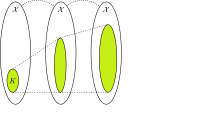
\includegraphics[width=\textwidth]{./figures/KP2.pdf}}
\only<3>{\includegraphics[width=\textwidth]{./figures/KP3.pdf}}
\only<4>{\includegraphics[width=\textwidth]{./figures/KP4.pdf}}
\only<5>{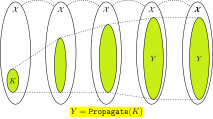
\includegraphics[width=\textwidth]{./figures/KP5.pdf}}
\only<6>{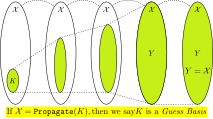
\includegraphics[width=\textwidth]{./figures/KP6.pdf}}
\end{figure}
\end{frame}

\begin{frame}{Naive Approach for GD}
Given a system of relations \((\mathcal{X}, \mathcal{R})\), where $|\mathcal{X}| = n$, 
is there any guess basis of size \(\leq m\)?

\onslide<2->{%
\begin{block}{Brute-force}
\footnotesize
\begin{itemize}
\item For \(k = 1 \rightarrow m\)
\begin{itemize}
\item For each subset \(K \subseteq \mathcal{X}\), where \(|K| = k\):
\begin{itemize}
\item If \(\texttt{Propagate(K)} = \mathcal{X}\) then return \(K\)
\end{itemize}
\end{itemize}
\end{itemize}
\end{block}
}
\onslide<3>{
\begin{itemize}
\item Time complexity \(\approx \sum_{k = 1}^{m}\binom{n}{k}\)\\
\item Exponential with respect to both $n$ and $m$
\end{itemize}
}
\end{frame}

\begin{frame}{Previous Works}
\begin{itemize}
\item Heuristic Approaches:
\begin{itemize}
\item[\faCheckCircleO] Dynamic programming: \cite{ahmadi2009heuristic}
\item[\faCheckCircleO] Dedicated algorithm for GD attaks on AES: \cite{bouillaguet2011automatic}
\end{itemize}
\item Using off-the-shelf solvers:
\begin{itemize}
\item[\faCheckCircle] \textcolor<2>{red}{MILP: \cite{cen2020minimizing}}
\item[\faCheckCircle] Gr\"obner basis: \cite{gd_groebner_2020}
\end{itemize}
\end{itemize}
\onslide<2>{We borrowed the idea introduced in \colorbox{gold}{\cite{cen2020minimizing}} to convert the GD problem to the CP/SAT problem.}
\end{frame}


\section{Constraint Programming Model for GD}
\sectionheader[\huge\color{tug}\faClockO]{Constraint Programming Model \\for GD}

\begin{frame}{Constraint Programming (CP)}
% \begin{itemize}
% \item Programming in CP refers to the arrangement of a plan
% \item For example the \href{https://developers.google.com/optimization/scheduling/employee_scheduling}{employee scheduling problem}
% \item 
In CP we specify the properties of the solution to be found:
\begin{itemize}
\item We define a set of variables: $\mathcal{X}$
\item We specify the domain of each variable: $\mathbb{F}_{2}, \mathbb{Z}, \mathbb{R}, \ldots$
\item We define a set of constraints: $\mathcal{C}$
\item We define an objective function (if it is required)
\end{itemize}
% \end{itemize}
\end{frame}

\begin{frame}[fragile]
\frametitle{CP Problem - Example}
\begin{figure}
\begin{center}
\only<1>{\includegraphics[width=0.5\textwidth]{./figures/austria.pdf}}
\only<2>{\includegraphics[width=0.5\textwidth]{./figures/austria_legend.pdf}}
\only<3>{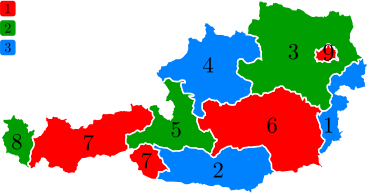
\includegraphics[width=0.5\textwidth]{./figures/austria3colored.pdf}}
\end{center}
\end{figure}
\pause
{\scriptsize
\begin{verbatim}
int: nc = 3;
array[1..9] of var 1..nc: r;
constraint r[1] != r[3]; constraint r[1] != r[6];
constraint r[2] != r[5]; constraint r[2] != r[6]; constraint r[2] != r[7];
constraint r[3] != r[9]; constraint r[3] != r[6]; constraint r[3] != r[4]; 
constraint r[4] != r[6]; constraint r[4] != r[5]; 
constraint r[5] != r[6]; constraint r[5] != r[7];  
constraint r[7] != r[8]; 
solve satisfy;
\end{verbatim}
\pause
\vspace{-0.4cm}
\begin{verbatim}
r = [3, 3, 2, 3, 2, 1, 1, 2, 1];
\end{verbatim}
}
\end{frame}

\begin{frame}{Main Steps of Our Approach}
Our method inspired from \cite{cen2020minimizing} has three main phases:
\begin{itemize}
\small
\item Convert the system of equations to a system of (implication and symmetric) relations
\item Convert the problem of finding a minimal guess basis for the system of relations to a CP problem or a sequence of SAT problems
\item Employ the off-the-shelf SAT/CP solvers to solve the problem
\end{itemize}
\end{frame}

\begin{frame}{Convert GD to a CP Problem}
\begin{columns}
\column{0.5\textwidth}
\begin{align*}
&r_{0}: [~\hlbox<4>{green}{x}, \hlbox<5>{yellow}{y}, z]&\\
&r_{1}: [z, w, \hlbox<5>{yellow}{y}]&\\
&r_{2}: [w, \hlbox<4>{green}{x}, u]&\\
\end{align*}
\only<3>{
\vspace{-1.5cm}
% \begin{align*}
% &\text{Fix the number of steps in }\\
% &X = \{~x_{i}, y_{i}, z_{i}, w_{i}, u_{i}: 0 \leq i \leq 2\}\\
% &\text{Domain: all variables are binary}\\
% &\text{Constraints}: \mathcal{C} \gets \emptyset
% \end{align*}
\begin{itemize}
\scriptsize
\item Fix the number of steps in knowledge propagation (e.g. 2 here)
\item $X = \{~x_{i}, y_{i}, z_{i}, w_{i}, u_{i}: 0 \leq i \leq 2\}$
\item $x_{i} = 1$ iff $x$ is known after the $i$th step of knowledge propagation, otherwise $x_{i} = 0$
\item $\mathcal{C} \gets \emptyset$
\end{itemize}
}
\only<4>{
\vspace{-1.5cm}
\begin{align*}
X \gets X &\cup \{~\hlbox<4>{green}{$x_{0, 0}$}, ~\hlbox<4>{green}{$x_{0, 1}$}\}&\\
\mathcal{C} \gets \mathcal{C} \cup &\{~\hlbox<4>{green}{$x_{0, 0}$} = y_{0} \wedge z_{0}\}&\\
\mathcal{C} \gets \mathcal{C} \cup &\{~\hlbox<4>{green}{$x_{0, 1}$} = w_{0} \wedge u_{0}\}&\\
\mathcal{C} \gets \mathcal{C} \cup &\{x_{1} = \hlbox<4>{green}{$x_{0, 0}$} \vee \hlbox<4>{green}{$x_{0, 1}$}\}&
\end{align*}
}
\only<5>{
\vspace{-1.5cm}
\begin{align*}
X \gets X &\cup \{~\hlbox<5>{yellow}{$y_{0, 0}$}, ~\hlbox<5>{yellow}{$y_{0, 1}$}\}&\\
\mathcal{C} \gets \mathcal{C} \cup &\{~\hlbox<5>{yellow}{$y_{0, 0}$} = x_{0} \wedge z_{0}\}&\\
\mathcal{C} \gets \mathcal{C} \cup &\{~\hlbox<5>{yellow}{$y_{0, 1}$} = z_{0} \wedge w_{0}\}&\\
\mathcal{C} \gets \mathcal{C} \cup &\{~\hlbox<5>{yellow}{$y_{1}$} =  \hlbox<5>{yellow}{$y_{0, 0}$} \vee \hlbox<5>{yellow}{$y_{0, 1}$}\}&
\end{align*}
}
\only<6>{
Do it for $z, w, u$ as well\\
}

\only<7>{
Do it for each transition in knowledge propagation
}

\only<8>{
All variables should be known at the last step:
\begin{equation*}
\mathcal{C} \gets \mathcal{C} \cup \{x_{2} \wedge y_{2} \wedge z_{2} \wedge w_{2} \wedge u_{2} = 1\}
\end{equation*}
}
\column{0.5\textwidth}
\only<2-9>{
\begin{figure}
\begin{tikzpicture}
\pgfmathsetmacro{\hd}{2};
\pgfmathsetmacro{\vd}{0.7};
\node[ellipse,draw] (s1) at (0, 0) {$x_{\onslide<3->{\color{red}{0}}}, ~ y_{\onslide<3->{\color{red}{0}}},  ~ z_{\onslide<3->{\color{red}{0}}}, ~ w_{\onslide<3->{\color{red}{0}}}, ~ u_{\onslide<3->{\color{red}{0}}}$};
\onslide<2->{
\node[ellipse,draw] (s2) at ($(s1) + (0, -2*\vd)$) {$x_{\onslide<3->{\color{red}{1}}}, ~ y_{\onslide<3->{\color{red}{1}}}, ~ z_{\onslide<3->{\color{red}{1}}}, ~ w_{\onslide<3->{\color{red}{1}}}, ~ u_{\onslide<3->{\color{red}{1}}}$};
\draw[>=latex, ->, rounded corners=20pt] (s1.0) -- ($0.5*(s1.0) + 0.5*(s2.0) + (0.5, 0)$) -- (s2.0);
}
\only<3>{
\node[ellipse,draw] (s3) at ($(s1) + (0, -4*\vd)$) {$x_{\color{red}{2}}, ~ y_{\color{red}{2}}, ~ z_{\color{red}{2}}, ~ w_{\color{red}{2}}, ~ u_{\color{red}{2}}$};
\draw[>=latex, ->, rounded corners=20pt] (s2.0) -- ($0.5*(s2.0) + 0.5*(s3.0) + (0.5, 0)$) -- (s3.0);
\node[ellipse] (s4) at ($(s1) + (0, -6*\vd)$) {$\textcolor{white}{x_{2}, ~ y_{2},~ z_{2}, ~ w_{2}, ~ u_{2}}$};
% \draw[>=latex, dashed, ->, rounded corners=20pt] (s3.0) -- ($0.5*(s3.0) + 0.5*(s4.0) + (0.5, 0)$) -- (s4.0);
}
\only<7->{
\node[ellipse,draw] (s3) at ($(s1) + (0, -4*\vd)$) {$x_{\color{red}{2}}, ~ y_{\color{red}{2}}, ~ z_{\color{red}{2}}, ~ w_{\color{red}{2}}, ~ u_{\color{red}{2}}$};
\draw[>=latex, ->, rounded corners=20pt] (s2.0) -- ($0.5*(s2.0) + 0.5*(s3.0) + (0.5, 0)$) -- (s3.0);
}
% \draw[->] (n1) -- (n2);
% \draw[->] (d1) -- (n1);
% \draw[->] (d2) -- (n2);
\end{tikzpicture}
\end{figure}
}
\only<10>{
\begin{figure}
\centering
\includegraphics[width=0.57\textwidth]{./figures/dg_example.pdf}
\end{figure}
}
\end{columns}
\only<9->{
\begin{align*}
\min~&x_{0} + y_{0} + z_{0} + w_{0} + u_{0}\\
s.t.& ~\text{all constraints in} ~ \mathcal{C} ~ \text{are satisfied}
\end{align*}
}
\end{frame}

\section{Autoguess}
\sectionheader[\huge\color{tug}\faGear]{Autoguess}
\begin{frame}{Autoguess}
\begin{figure}
\centering
\includegraphics[width=\textwidth]{./figures/autoguess_design.pdf}
\end{figure}
\end{frame}

\begin{frame}
\frametitle{Autoguess - Simple User Interface}
\begin{columns}
\column{0.5\textwidth}
\only<1>{
{\footnotesize
\begin{align*}
\quad \left \{ \begin{array}{lr}
\textcolor<2>{blue}{F(u + v) \oplus G(x) \oplus y \oplus (z \lll 7)} &= c_{1}\\
\textcolor<2>{blue}{G(u \oplus w) + (y \lll 3) + z} &= c_{2}\\
\textcolor<2>{blue}{F(w \oplus x) + y \oplus z} &= c_{3}\\
\textcolor<2>{blue}{F(u) \oplus G(w + z)} &= c_{4}\\
\left(\textcolor<2>{red}{F(u) \times G(w\lll 7)}\right) + \textcolor<2>{blue}{H(z\oplus v)} &= c_{5}\\
\end{array} \right.
\end{align*}
}
}
\only<2->{
{\footnotesize
Input file (\texttt{relations.txt}):
}
\begin{figure}
\begin{flushleft}
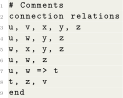
\includegraphics[scale=1]{figures/autoguess_inputfile.pdf}
\end{flushleft}
\end{figure}
}
\column{0.5\textwidth}
\only<3>{
{\footnotesize
Output:
}
\begin{figure}
\centering
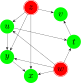
\includegraphics[width=0.65\textwidth]{figures/autoguess_usage.pdf}
\end{figure}
}
\end{columns}
\vspace{1.5cm}
\only<2>{
{\footnotesize
Run Autoguess:
}

{\scriptsize
\colorbox{darkgray}{\textcolor{white}{\texttt{python3 autoguess.py -i relations.txt --maxsteps 5 --solver cp}}}
}
}
\end{frame}

\begin{frame}{GD Attack on Block Ciphers (1 round of AES)}
\only<1>{%
\begin{figure}
\begin{center}
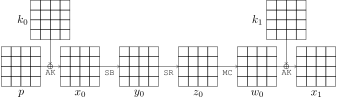
\includegraphics[]{./figures/aes1rgd1.pdf}
\end{center}
\end{figure}
}
\only<2>{%
\begin{figure}
\begin{center}
\includegraphics[]{./figures/aes1rgd2.pdf}
\end{center}
\end{figure}
}
% \only<3>{%
% \begin{figure}
% \begin{center}
% \includegraphics[]{./figures/aes1rgd3.pdf}
% \end{center}
% \end{figure}
% }
\only<3>{
\begin{figure}
\centering
\includegraphics[width=0.78\textwidth]{./figures/aes_1_round_gd_dg.pdf}
\end{figure}
\vspace{-0.2cm}
\scriptsize
\centering
Found in \colorbox{gold}{0.02 seconds} on a \texttt{2.8 GHz i7-1165G7 CPU}
}
\end{frame}


\begin{frame}{GD Attack on Block Ciphers (3 Rounds of AES)}
\begin{figure}
\centering
\includegraphics[width=0.78\textwidth]{figures/aes_3_rounds_gd_dg.pdf}
\end{figure}
\vspace{-0.2cm}
\scriptsize
\centering
Found in \colorbox{gold}{34.51 seconds} on a \texttt{2.8 GHz i7-1165G7 CPU}
\end{frame}

\begin{frame}{GD Attack on Stream Ciphers (KCipher-2)}
\only<1>{
\begin{figure}
\centering
\includegraphics[scale=0.35]{figures/kcipher2.pdf}
\end{figure}
\centering
\scriptsize
\vspace{-0.2cm}
\href{https://www.iso.org/standard/54532.html}{ISO/IEC 18033-4}
}
\only<2>{
\begin{figure}
\centering
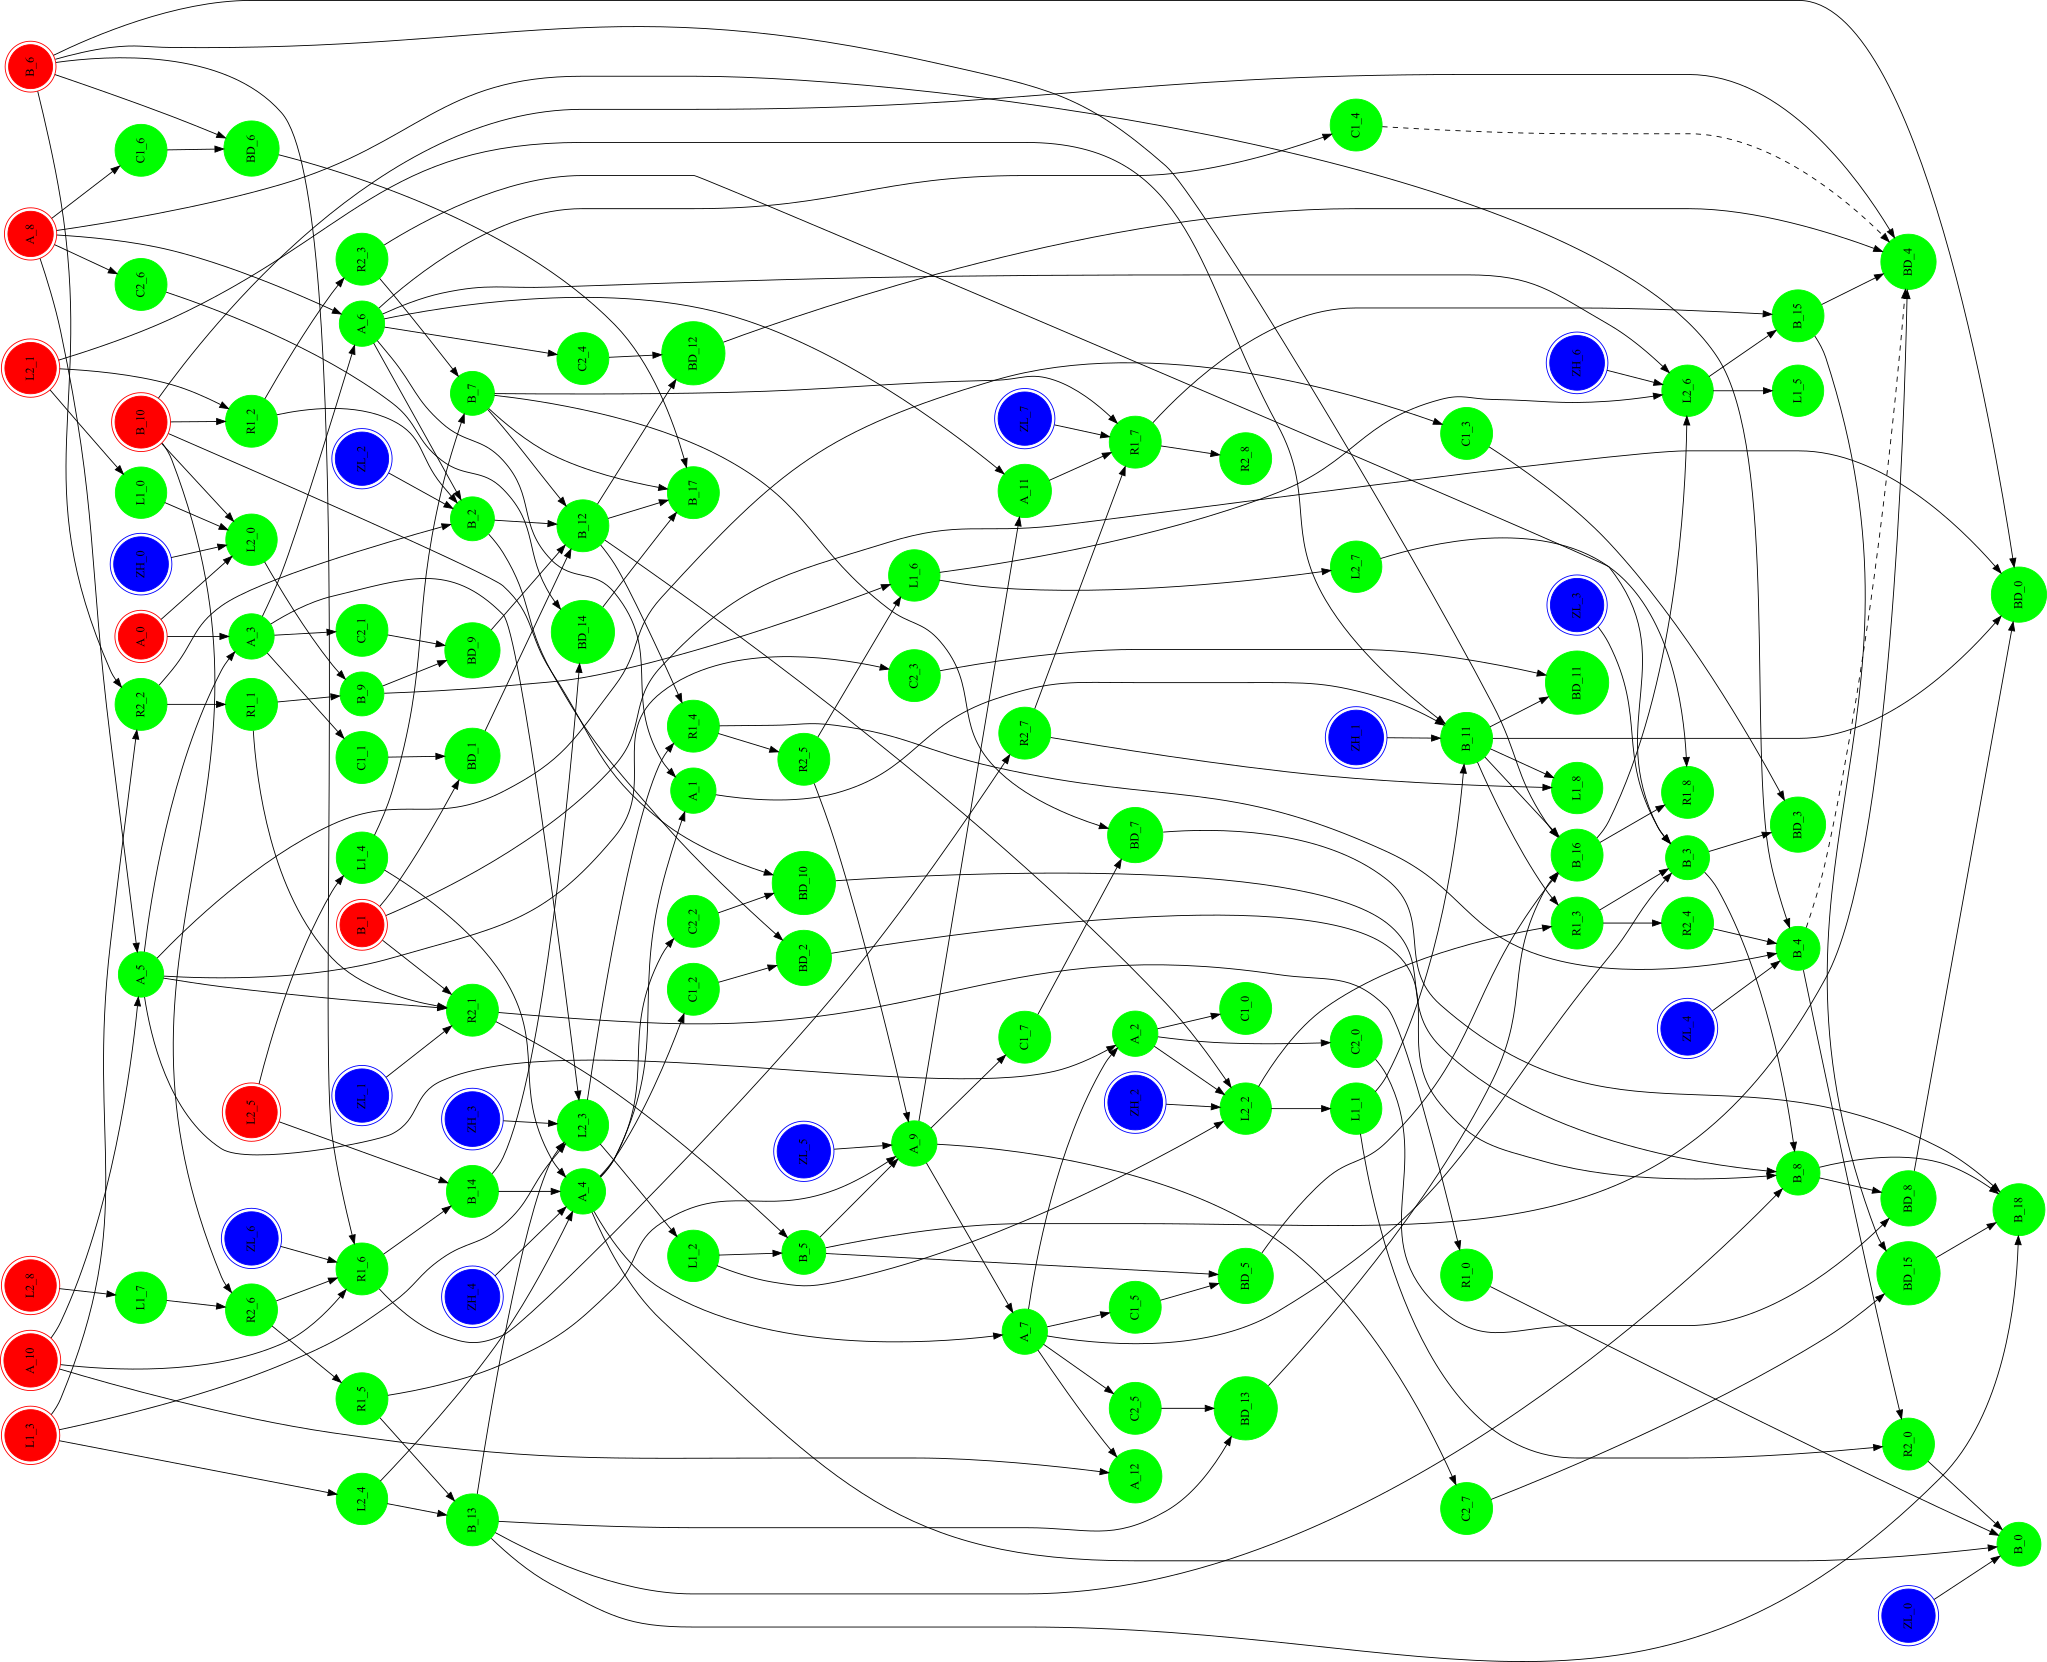
\includegraphics[width=0.65\textwidth]{figures/kcipher2_8clks_10g_19s_gd_dg.pdf}
\end{figure}
\vspace{-0.2cm}
\scriptsize
\centering
Found in \colorbox{gold}{7 seconds} on a \texttt{2.8 GHz i7-1165G7 CPU}
}
\end{frame}

\section{Key-Bridging (KB)}
\sectionheader[\huge\color{tug}\faRoad]{Key-Bridging (KB)}
\begin{frame}{Key-Bridging (KB)}
\begin{figure}
\centering
\only<1>{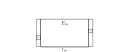
\includegraphics[width=\textwidth]{./figures/KB1.pdf}}
\only<2>{
\includegraphics[width=\textwidth]{./figures/KB2.pdf}}
\only<3>{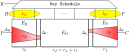
\includegraphics[width=\textwidth]{./figures/KB3.pdf}}
\end{figure}
\onslide<3>{
\begin{itemize}
\scriptsize
\item We want to determine a subset of sub-key bits: \(B \cup F\)
% \vspace{-0.2cm}
\item Key schedule implies some relations between the sub-key bits in \(B\cup F\)
% \vspace{-0.2cm}
\item \textcolor{red}{Find a minimal guess basis for $B \cup F$ (not for the entire set of variables)}
\end{itemize}
}
\end{frame}

\begin{frame}{$\mathcal{DS}$-MITM Attacks On SKINNY and TWINE}
\begin{itemize}
\item We combined our CP-based method for KB with CP-based method to search for distinguishers
\item We applied our method to optimize \(\mathcal{DS}\)-MITM attack on SKINNY \cite{skinny} and TWINE \cite{suzaki2011twine}
\end{itemize}
\begin{table}[!]
\centering
  \resizebox{\textwidth}{!}{\begin{tabular}{@{}lccccccl@{}}
    \hline
    Cipher          & $\#$Rounds & Data        & Memory                     & Time                & Attack              & Setting & Reference\\ \hline
    SKINNY-128-256 & 19         & $2^{96}$ CP & $2^{210.99}$               & $2^{238.26}$        & $\mathcal{DS}$-MITM & ST      & This paper\\
    SKINNY-64-192  & 21         & $2^{60}$ CP & $2^{133.99}$               & $2^{186.63}$        & $\mathcal{DS}$-MITM & ST      & This paper\\
    SKINNY-64-128  & 18         & $2^{32}$ CP & $2^{61.91}$                & $2^{126.32}$        & $\mathcal{DS}$-MITM & ST      & This paper\\ \hline
    TWINE-80       & 20         & $2^{32}$ CP & $\boldsymbol{2^{62.91}}$   & $2^{76.92}$         & $\mathcal{DS}$-MITM &  -      & This paper\\
    TWINE-80       & 20         & $2^{32}$ CP & $2^{82.91}$                & $2^{77.44}$         & $\mathcal{DS}$-MITM &  -      & \cite{shi2018programming}\\ \hline		
\end{tabular}}
\end{table}
\end{frame}


\section{Conclusion}
\sectionheader[\huge\color{tug}\faClockO]{Conclusion}
\begin{frame}{Our Contributions - I}
\begin{itemize}
\item[\faCheckCircleO] We introduced two new encoding methods for GD technique (CP \& SAT)
\pause
\item[\faCheckCircleO] We provided the open-source tool Autoguess integrating our new methods as well as almost all of the previous methods for GD technique
\pause
\item[\faCheckCircleO] We applied our tool on a wide variety of symmetric primitives:
\begin{itemize}
\scriptsize
\item Improving the GD attack on ZUC \cite{zuc128_specification, zuc256_specification}
\item Rediscovering the GD attack on 3 rounds of AES in less than a minute
\end{itemize}
\item[\faCheckCircleO] We applied Autoguess to find key-bridges in key recovery attacks on block ciphers
\end{itemize}
\end{frame}
\begin{frame}{Our Contributions - II}
\begin{itemize}
\footnotesize
\item[\faCheckCircleO] We combined our CP-based approach for key-bridging with the CP-based methods to search for distinguishers,
and introduced a unified method to find key-recovery friendly distinguishers:
\end{itemize}
\begin{center}
\vspace{0.5cm}
\pause
{\large Thanks for your attention!}
\vspace{0.5cm}

\faGithub: \url{https://github.com/hadipourh/autoguess}\\
\vspace{0.2cm}
\faArchive: \url{https://ia.cr/2021/1529}
\end{center}
\end{frame}

%%%%%%%%%%%%%%%%%%%%%%%%%%%%%%%%%%%%%%%%%%%%%%%%%%%%%%%%%%%%%%%%%%%%%%%%%%%%

\begin{frame}[allowframebreaks]{Bibliography}
  \printbibliography
\end{frame}

\begin{filecontents*}[overwrite]{\jobname.bib}

@article{ahmadi2009heuristic,
  title={Heuristic guess-and-determine attacks on stream ciphers},
  author={Ahmadi, Hadi and Eghlidos, Taraneh},
  journal={IET Information Security},
  volume={3},
  number={2},
  pages={66--73},
  year={2009},
  publisher={IET}
}

@article{cen2020minimizing,
title={Minimizing Deduction System and its Application},
author={Cen, Zhe and Feng, Xiutao and Wang, Zhangyi and Cao, Chunping},
journal={arXiv preprint arXiv:2006.05833},
url={https://arxiv.org/abs/2006.05833},
year={2020}
}

@inproceedings{bouillaguet2011automatic,
  title={Automatic search of attacks on round-reduced {AES} and applications},
  author={Bouillaguet, Charles and Derbez, Patrick and Fouque, Pierre-Alain},
  booktitle={Advances in Cryptology -- CRYPTO 2011},
  pages={169--187},
  year={2011},
  organization={Springer}
}

@article{gd_groebner_2020,
	title={A fault attack on {KCipher-2}},
	author={Danner, J and Kreuzer, M},
	journal={International Journal of Computer Mathematics: Computer Systems Theory},
	pages={1--22},
	year={2020},
	publisher={Taylor \& Francis}
}

@inproceedings{skinny,
  title={{The SKINNY family of block ciphers and its low-latency variant MANTIS}},
  author={Beierle, Christof and Jean, J{\'e}r{\'e}my and K{\"o}lbl, Stefan and Leander, Gregor and Moradi, Amir and Peyrin, Thomas and Sasaki, Yu and Sasdrich, Pascal and Sim, Siang Meng},
  booktitle={Advances in Cryptology -- CRYPTO 2016},
  pages={123--153},
  year={2016},
  organization={Springer}
}

@inproceedings{suzaki2011twine,
  title={Twine: A lightweight, versatile block cipher},
  author={Suzaki, Tomoyasu and Minematsu, Kazuhiko and Morioka, Sumio and Kobayashi, Eita},
  booktitle={ECRYPT workshop on lightweight cryptography},
  volume={2011},
  year={2011}
}

@inproceedings{shi2018programming,
	title={Programming the {Demirci}-{Sel{\c{c}}uk} meet-in-the-middle attack with constraints},
	author={Shi, Danping and Sun, Siwei and Derbez, Patrick and Todo, Yosuke and Sun, Bing and Hu, Lei},
	booktitle={Advances in Cryptology -- ASIACRYPT 2018},
	pages={3--34},
	year={2018},
	organization={Springer}
}

@article{zuc128_specification,
	author    = {ETSI/SAGE},
	title     = {Specification of the 3GPP confidentiality and integrity algorithms
	{128-EEA3} and {128-EIA3}: {ZUC} specification},
	journal   = {ETSI/SAGE, Document 2, Version 1.6},
	year      = {2011}
}

@article{zuc256_specification,
	author    = {ZUC Design Team},
	title     = {The {ZUC}-256 Stream Cipher},
	year      = {2018},
	note         = {\url{http://www.is.cas.cn/ztzl2016/zouchongzhi/201801/W020180126529970733243.pdf}}
}

\end{filecontents*}

\end{document}
